%--------------------------------------------------------------------------------------%--------------------------------------------------------------------------------------
%
%  Global settings, dont change it! (excapt additional \usepackage commands)
%  Always use PDFLatex!
%
%--------------------------------------------------------------------------------------%--------------------------------------------------------------------------------------
\documentclass[a4paper, 12pt, oneside, BCOR1cm,toc=chapterentrywithdots]{scrbook}

\usepackage{graphicx}           % use for pdfLatex
\usepackage{makeidx} % f\"{u}r Benutzung des Befehls \printindex
\usepackage[colorlinks=false]{hyperref}
\usepackage{tocbibind}
\usepackage{blindtext}
\usepackage{subfigure} 
\usepackage{acronym}

\hypersetup{%
bookmarksnumbered=true, hyperindex=true,
%
%Im Acrobat Reader Subtitel 1. Ebene anzeigen
bookmarksopen=true, bookmarksopenlevel=1,
%
pdfborder=0 0 0 % Keine Box um die Links!
}

% --------------------------------------------------------------
% Force Tables and List to be added in Table of Content
% --------------------------------------------------------------

\renewcommand*{\tableofcontents}{%
  	\begingroup
  	\tocsection
  	\tocfile{\contentsname}{toc}
  	\endgroup
}
\renewcommand*{\listoffigures}{%
  	\begingroup
  	\tocsection
  	\tocfile{\listfigurename}{lof}
  	\endgroup
}
\renewcommand{\listoftables}{
	\begingroup
	\tocsection
	\tocfile{\listtablename}{lot}
	\endgroup
}
\begin{document}

%--------------------------------------------------------------------------------------%--------------------------------------------------------------------------------------
%
%  Here starts the userspace !
%
%--------------------------------------------------------------------------------------%--------------------------------------------------------------------------------------

%--------titlepage
\begin{titlepage}

{
    \begin{center}
        \raisebox{-1ex}{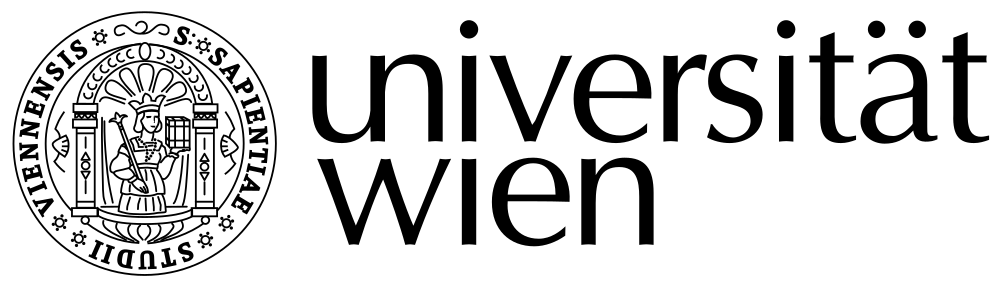
\includegraphics[scale=0.2]{Logo.png}}\\
    \end{center}
    \vspace{1.5cm}
}

\begin{center}


\LARGE{\textbf{MASTERARBEIT}}\\
\vspace{1.5cm}

\small{Titel}\\
\Large{\textbf{Automatic Generation and Translation of Process Collaboration Models to BPMN/XML}}\\ 
\vspace{2cm}
\small {verfasst von}\\
\large Frederik Bischoff BSc\\
\vspace{0.7cm}
\small angestrebter akademischer Grad\\
\large Diplom-Ingenieur (Dipl.-Ing.)\\
\end{center}
\vspace{3cm}
\small 
Wien, 2017\\
\vspace{2cm}\\
\begin{tabbing}
Studienkennzahl lt. Studienblatt: \= \= \= A 066 926\\
Studienrichtung lt. Studienblatt: \> Masterstudium Wirtschaftsinformatik\\
Betreut von: \> Univ.-Prof. Dipl.-Math. Dr. Stefanie Rinderle-Ma\\
\end{tabbing}

\end{titlepage}


%---------------------------------------------------------
% Table of Contents, List of figures, List of Tables
%---------------------------------------------------------

\tableofcontents
\listoffigures
\listoftables

%---------------------------------------------------------
% List of Abbreviations
%---------------------------------------------------------
\twocolumn
\addchap{List of Abbreviations}
\begin{acronym}[Bash]
 \acro{KDE}{K Desktop Environment}
 \acro{SQL}{Structured Query Language}
 \acro{Bash}{Bourne-again shell}
 \acro{JDK}{Java Development Kit}
 \acro{VM}{Virtuelle Maschine}
 \acro{I2C}[I²C]{Inter-Integrated Circuit}
 \acro{KDE}{K Desktop Environment}
 \acro{SQL}{Structured Query Language}
 \acro{Bash}{Bourne-again shell}
 \acro{JDK}{Java Development Kit}
 \acro{VM}{Virtuelle Maschine}
 \acro{I2C}[I²C]{Inter-Integrated Circuit}
 \acro{KDE}{K Desktop Environment}
 \acro{SQL}{Structured Query Language}
 \acro{Bash}{Bourne-again shell}
 \acro{JDK}{Java Development Kit}
 \acro{VM}{Virtuelle Maschine}
 \acro{I2C}[I²C]{Inter-Integrated Circuit}
 \acro{KDE}{K Desktop Environment}
 \acro{SQL}{Structured Query Language}
 \acro{Bash}{Bourne-again shell}
 \acro{JDK}{Java Development Kit}
 \acro{VM}{Virtuelle Maschine}
 \acro{I2C}[I²C]{Inter-Integrated Circuit}
 \acro{KDE}{K Desktop Environment}
 \acro{SQL}{Structured Query Language}
 \acro{Bash}{Bourne-again shell}
 \acro{JDK}{Java Development Kit}
 \acro{VM}{Virtuelle Maschine}
 \acro{I2C}[I²C]{Inter-Integrated Circuit}
 \acro{KDE}{K Desktop Environment}
 \acro{SQL}{Structured Query Language}
 \acro{Bash}{Bourne-again shell}
 \acro{JDK}{Java Development Kit}
 \acro{VM}{Virtuelle Maschine}
 \acro{I2C}[I²C]{Inter-Integrated Circuit}
\end{acronym}

\onecolumn
%---------------------------------------------------------
% Here starts the real work
%---------------------------------------------------------

\chapter{Introduction}
In the research field of business process models and techniques, researchers can only rely on a repository of centralized, intra-organizational processes to support their work. But regarding decentralized, cross-organizational models, they face the problem that there is a lack of available model examples. Within the scope of this work, this lack is aimed to be tackled. Thereby, the main objective is to build a repository of distributed and collaborative process models by developing and implementing an automatic generation process for business process collaborations. The generation process must thereby ensure soundness, consistency and compatibility of the resulting models. Additionally, it should also allow the generation of models which comply to imposed compliance rules. At last, to ensure the executability of the auto-generated models by process engines, an additional goal of this work is to develop a transformation of the utilized RPST\footnote{Refined Process Structure Tree } representation to BPMN\footnote{Business Process Model and Notation - http://www.bpmn.org/}. These requirements ensure that the repository can then be used for further research, such as change management or process mining of collaborative processes. Based on those objectives, the following research questions are derived:

\begin{itemize}
\item \textit{RQ-1}: How to build a repository of collaboration process models that can be used as support for further research in this field?
\item \textit{RQ-2}: How to ensure that the resulting process models in this repository are correct in terms of consistency, compatibility and compliability? Which process flow perspectives and compliance rule patterns should be supported regarding compliability? 
\item \textit{RQ-3}: How to transform a collaborative process represented as an RPST into an executable form?
\end{itemize}

This work is part of the CRISP\footnote{http://gruppe.wst.univie.ac.at/projects/crisp/} project (ICT15-072) funded by the Vienna Science and Technology Fund (WWTF). The implementation of the prototype is integrated in an already existing framework. The main research within the project is to analyze flexibility and adaptivity of collaborative business processes at design time as well as at runtime. Regarding consistency and correctness of collaborative business processes, the propagation of a process change over all process participants is one of the main challenges the project tries to tackle. Furthermore, the impact of compliance rules imposed on collaborative business scenarios is analyzed as well as the issue of ensuring business compliance by considering the privacy and autonomy of the involved business partners.\\

This work is structured as followed. First, a brief overview of related work is given in Chapter \ref{chap:relwork}, followed by an introduction into process collaborations represented in BPMN by explaining the different model views in Chapter \ref{chap:theo}. Then the concept of the automatic collaboration process generator is introduced in Chapter \ref{chap:conception}. Thereby the approach, the possibility of influencing the outcome and the therefor necessary components are explained. Afterwards, in Chapter \ref{chap:impl}, the adaption of the RPST for the internal process model representation is explained as well as the class structure and data models of the implemented components. The performance of the implemented generation process depending on different parameter settings is then examined in Chapter \ref{chap:analysis}. Finally, the work is concluded in Chapter \ref{chap:concl}.  % Load Data from File intro.tex

\chapter{Tables}
% Example of, how to use a Table

\blindtext[1]

\begin{center}
\begin{tabular}{|c|c|c|c|}
\hline
Wert 1 & Wert 2 & Wert 3 & Wert 4\\
in Einheit1 & in Einheit2 & in Einheit3 & in Einheit4 \\
\hline
192 & 80& 0.3153 & 0.4900\\
500 & 120& 0.1229& 0.1787\\
1000 & 120& 0.0680& 0.0880\\
2000 & 120& 0.0361& 0.0441\\
5000 & 140& 0.0256& 0.0305\\
5000 & 164& 0.0343& 0.0880\\
\hline
\end{tabular}
\captionof{table}{This is the caption of the table}
\label{tab:table1}
\end{center}

\blindtext[3] % Load Data from File example_tables

\chapter{Figures}
% Example of, how to use figures

\blindtext

\begin{figure}[h]
\centering
\includegraphics[width=0.6\textwidth]{TU_Chemnitz_positiv_gruen.pdf}
\caption{Graphic 1}
\label{fig:pic0}
\end{figure}

\blindtext
\blindtext

\begin{figure}[h]
    \subfigure[This is the first graphic]{\includegraphics[width=0.49\textwidth]{TU_Chemnitz_positiv_gruen.pdf} \label{fig:pic1}}
    \subfigure[This is the secound graphic]{\includegraphics[width=0.49\textwidth]{TU_Chemnitz_positiv_gruen.pdf}\label{fig:pic2}}
\caption{This is the caption of the whole graphic}
\end{figure}

\blindtext

 % Load Data from File example_figures

\chapter{Referencing}
% Alternativ just write your text under \chapter like this example

\blindtext \cite{autorenrichtlinien}

\blindtext \footnote{Here is an area for your Notes}

\blindtext \footnote{\cite{lnilatex} Seite 11}
\blindtext \cite{lnilatex}
\blindtext \cite{autorenrichtlinien}


\chapter{Subchapter}

\section{sub 1}
\blindtext[3]
\section{sub 2}
\blindtext[3]
\subsection{sub 2.1}
\blindtext[3]

\subsection{sub 2.2}
\blindtext[3]

%---------------------------------------------------------
% bibliography based on Springer Design
%---------------------------------------------------------

\bibliographystyle{splncs03}
\bibliography{bibliography}

\printindex

\end{document}
